\documentclass[conference]{IEEEtran}
\IEEEoverridecommandlockouts
% The preceding line is only needed to identify funding in the first footnote. If that is unneeded, please comment it out.
\usepackage{cite}
\usepackage{amsmath,amssymb,amsfonts}
\usepackage{algorithmic}
\usepackage{graphicx}
\usepackage{textcomp}
\usepackage{subcaption}
\usepackage[spanish]{babel}
\usepackage{hyperref}
\usepackage{array}
\usepackage{listings}
\usepackage{float}
\usepackage{xcolor}
\definecolor{codegreen}{rgb}{0,0.6,0}
\definecolor{codegray}{rgb}{0.5,0.5,0.5}
\definecolor{codepurple}{rgb}{0.58,0,0.82}
\definecolor{backcolour}{rgb}{0.95,0.95,0.92}
\lstdefinestyle{mystyle}{ 
    commentstyle=\color{codegreen},
    keywordstyle=\color{magenta},
    numberstyle=\tiny\color{codegray},
    stringstyle=\color{codepurple},
    basicstyle=\ttfamily\footnotesize,
    breakatwhitespace=false,         
    breaklines=true,                 
    captionpos=b,                    
    keepspaces=true,                 
    showspaces=false,                
    showstringspaces=false,
    showtabs=false,                  
    tabsize=2
}
\lstset{style=mystyle}
\usepackage{comment}

\def\BibTeX{{\rm B\kern-.05em{\sc i\kern-.025em b}\kern-.08em
    T\kern-.1667em\lower.7ex\hbox{E}\kern-.125emX}}
\begin{document}

\title{Proyecto final: Análisis de sargazo \\
{\large {\vspace{0.7cm} Reconocimiento de Patrones - 0757 \\ \vspace{0.1cm} \textit{Facultad de Ingeniería, }  \\ \textsc{Universidad Nacional Autónoma de México}}}
\thanks{Reconocimiento de Patrones - 0757 \\ I.I.M.A.S - U.N.A.M.}
}

\author{
    \IEEEauthorblockN{Martínez Ostoa N.I. \\ \#315618648}
    \IEEEauthorblockA{\textit{Ing. en Computación} \\
    \textit{Facultad de Ingeniería, UNAM}\\
    Ciudad de México, México \\
    nestor.martinez@iimas.unam.mx}
    \and
    \IEEEauthorblockN{Ramírez Bondi J. A. \\ \#314634825}
    \IEEEauthorblockA{\textit{Ing. en Computación} \\
    \textit{Facultad de Ingeniería, UNAM}\\
    Ciudad de México, México \\
    alejandrobondi@me.com}
    \and
    \IEEEauthorblockN{\textbf{Profesores:}}
    \IEEEauthorblockA{Dr. Boris Escalante Ramírez \\ Dra. Jimena Olveres Montiel\\ \textit{I.I.M.A.S. - U.N.A.M.}}
}

\maketitle

\begin{abstract}

\end{abstract}

% -------------------------------------------------
% -------------------------------------------------
% -------------------------------------------------
\section{Objetivo}
\begin{itemize}
    \item Realizar un análisis de imágenes tomadas en distintos momentos de una playa en Puerto Morelos, Quintana Roo para detectar la presencia de sargazo en el océano y ayudar en la estimación del arribo de este elemento que afecta al turismo y demás actividades económicas.
    \item A partir del análisis, realizar alguna de las siguientes actividades concretas:
    \begin{itemize}
        \item Detección del sargazo
        \item Segmentación de las manchas del sargazo
        \item Seguimiento del movimiento del sargazo
        \item Cuantificación, en píxeles, del sargazo.
    \end{itemize}
\end{itemize}

% -------------------------------------------------
% -------------------------------------------------
% -------------------------------------------------
\section{Introducción}

La llegada atípica de sargazo a las playas mexicanas y el Caribe ha provocado afectaciones económicas significativas en las entidades cuya economía está mayoritariamente basada en los ingresos por actividades turísticas.

Desde que se comenzó a contar con tecnología satelital, el monitoreo de las costas, corrientes y estado del tiempo se realizaba con imágenes obtenidas desde el espacio. Sin embargo, esta técnica de observación no ha sido muy eficaz para vigilar la llegada de sargazo a las playas mexicanas de manera precisa. Es decir, las imágenes satelitales nos permiten conocer si grandes masas de dicha alga van camino hacia el territorio mexicano, pero no nos permiten determinar con mayor precisión la playa a la que dicha biomasa llegará.

Lo anterior, nos ha llevado a pensar en una solución---mediante el análisis de imágenes---que pueda escalarse a una gran cantidad de playas, en especial aquellas con presencia turística, para mejorar la respuesta de las autoridades en el retiro y monitoreo del sargazo.

Este proyecto propone el desarrollo de modelos diversos para cuantificar, detectar y dar seguimiento a los cuerpos de sargazo a una playa ubicada en Puerto Morelos, Quintana Roo. El trabajo inicial, consistió en la recolección de imágenes con vista a la playa y el mar---por donde habitualmente llegan grandes cantidades de sargazo---por el equipo estacionado en una sede de la UNAM.

A partir de la secuencia de imágenes se realizó el procesamiento pertinente sobre las mismas, se segmentaron mediante diversas técnicas y se etiquetó por clases cada uno de los segmentos obtenidos. Finalmente, con la información antes mencionada, se entrenaron los modelos que se han considerado pertinentes para poder detectar si una imagen cuenta con la presencia de sargazo o no.

Así, se espera que este tipo de acercamientos para resolver la serie de problemas que se suscitan con la presencia del sargazo en las playas y mares del territorio mexicano, puedan ser atacados mediante el uso de imágenes obtenidas en puntos estratégicos distribuidos a lo largo de la zona costera afectada. Además, esta técnica ayudaría a tener información en tiempo real y dar respuesta lo antes posible---siendo fundamental la celeridad puesto que el sargazo entra en estado de descomposición y emite un olor muy desagradable para las personas ubicadas sobre la playa.




% -------------------------------------------------
% -------------------------------------------------
% -------------------------------------------------
\section{Desarrollo}
Para resolver los objetivos planteados en este proyecto diseñamos una arquitectura que consta de las siguientes fases:

\begin{enumerate}
    \item Muestreo de imágenes
    \item División de imágenes en imágenes de entrenamiento y prueba
    \item Clasificación de imágenes
    \item Extracción de características relevantes
    \item Entrenamiento y evaluación de modelos 
\end{enumerate}

\subsection{Muestreo de imágenes}
Del \textit{pool} original de imágenes, decidimos seleccionar las imágenes más representativas para identificar el sargazo. Nuestro base de imágenes constó de 11 imágenes: 

\begin{itemize}
    \item \verb|1622134320.Thu.May.27_16_52_00.GMT.2021|
    \item \verb|1622134380.Thu.May.27_16_53_00.GMT.2021|
    \item \verb|1622134620.Thu.May.27_16_57_00.GMT.2021|
    \item \verb|1622138440.Thu.May.27_18_00_40.GMT.2021|
    \item \verb|1622144920.Thu.May.27_19_48_40.GMT.2021|
    \item \verb|1622157720.Thu.May.27_23_22_00.GMT.2021|
    \item \verb|1622732400.Thu.Jun.03_15_00_00.GMT.2021|
    \item \verb|1622732880.Thu.Jun.03_15_08_00.GMT.2021|
    \item \verb|1623441780.Fri.Jun.11_20_03_00.GMT.2021|
    \item \verb|1623442440.Fri.Jun.11_20_14_00.GMT.2021|
    \item \verb|1623442740.Fri.Jun.11_20_19_00.GMT.2021|
\end{itemize}

A continuación se muestran dos de estas imágenes:

\begin{figure}[H]
    \centering
    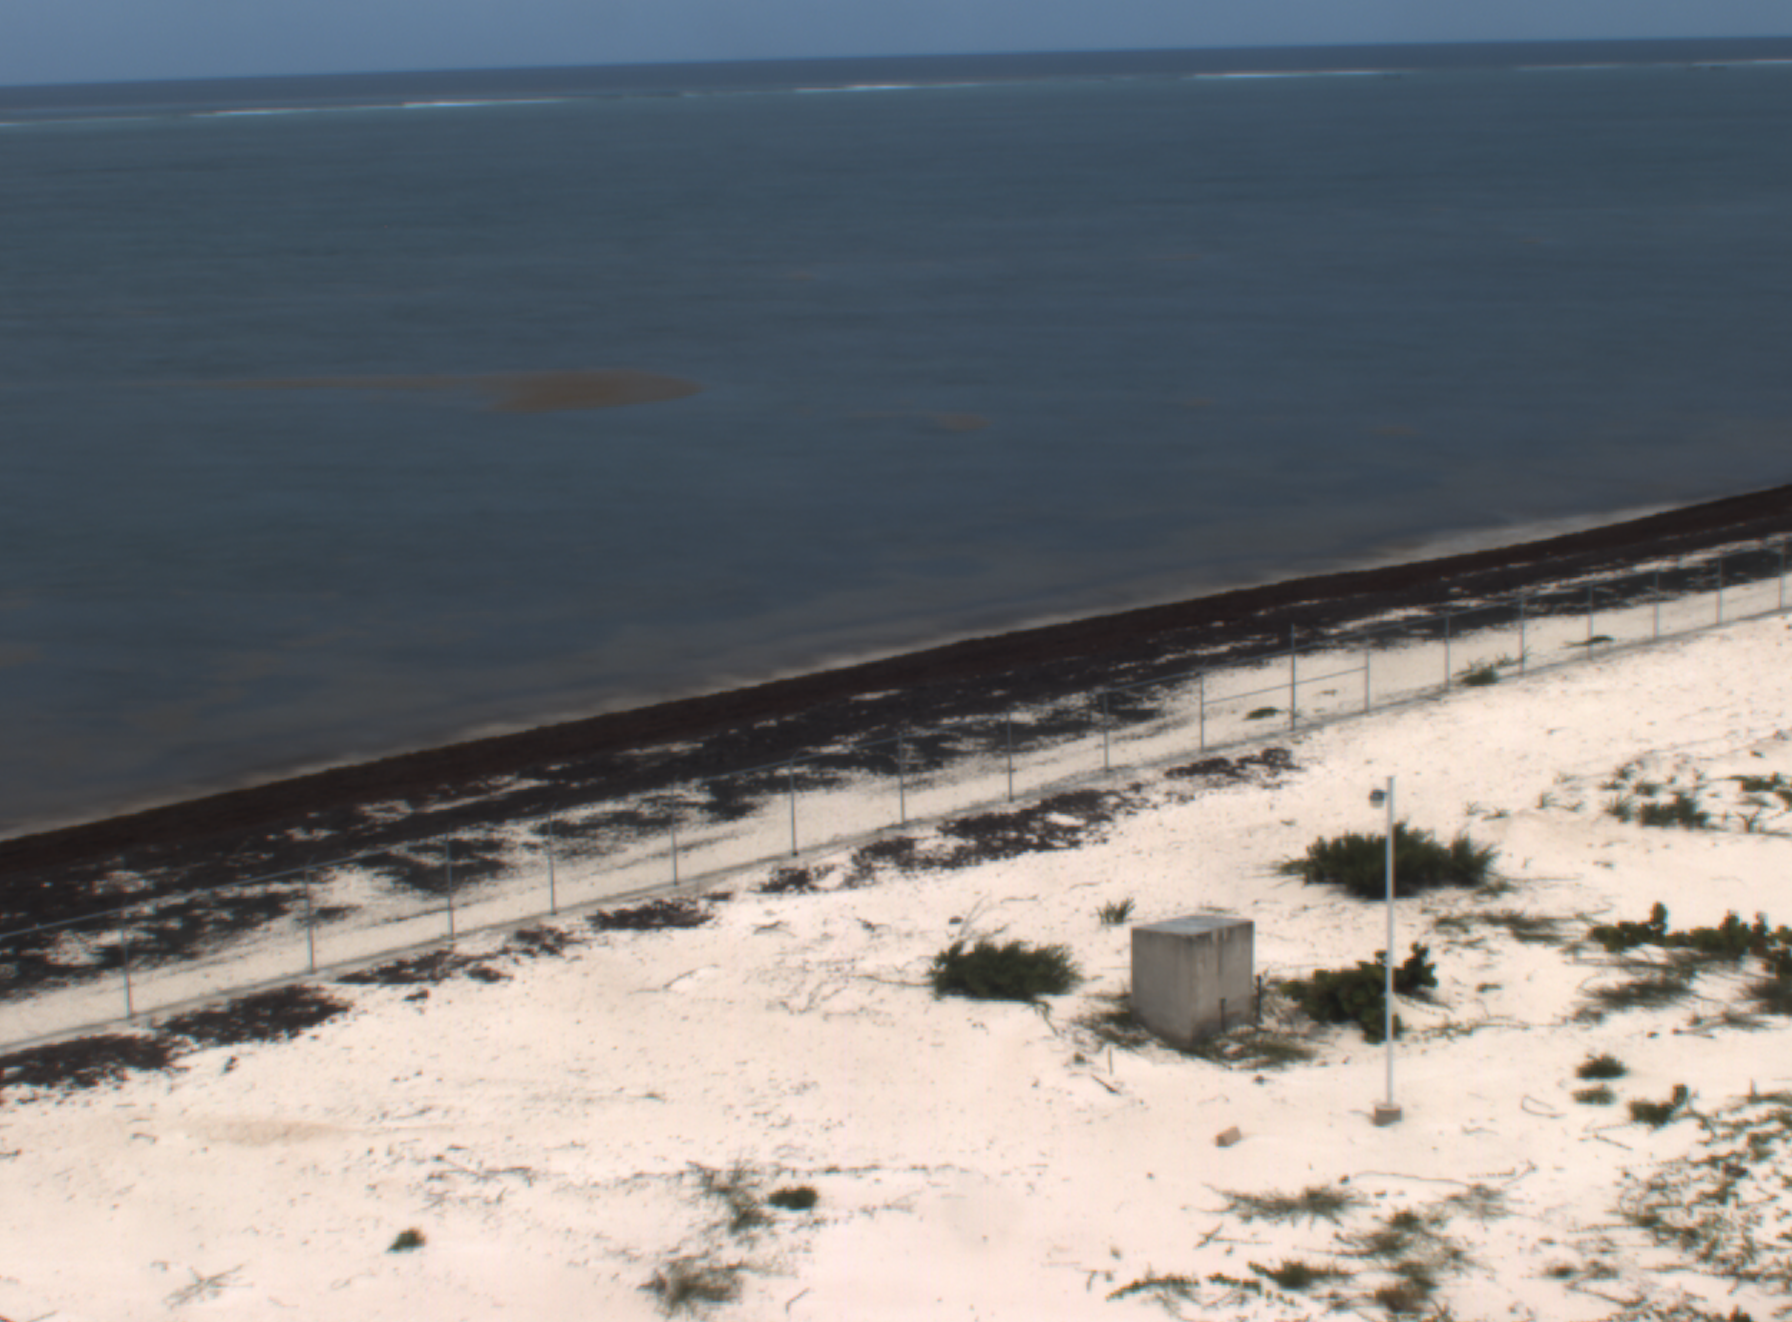
\includegraphics[scale=0.13]{imgs/selected_img_2.png}
    \caption{1622138440.Thu.May.27\_18\_00\_40.GMT.2021}
\end{figure}

\begin{figure}[H]
    \centering
    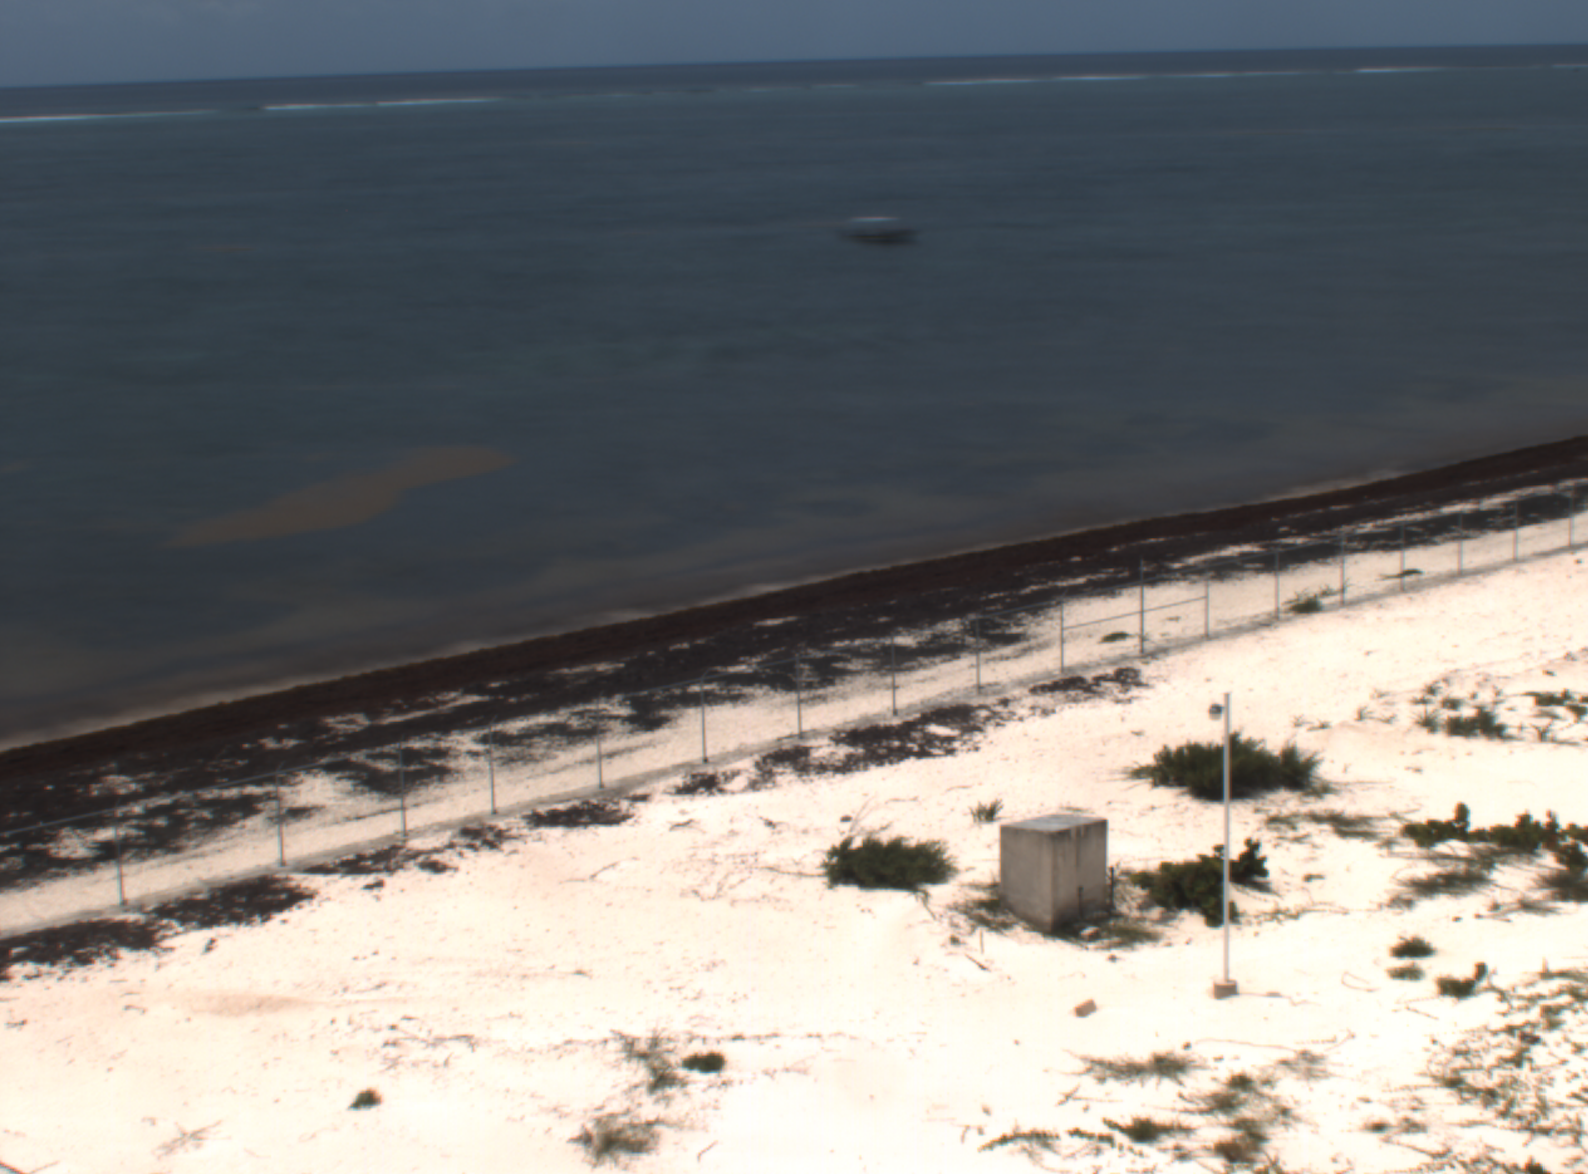
\includegraphics[scale=0.13]{imgs/selected_img_1.png}
    \caption{1622134380.Thu.May.27\_16\_53\_00.GMT.2021}
\end{figure}


\subsection{División de imágenes en imágenes de entrenamiento y prueba}
Para esta sección, lo que hicimos fue lo siguiente:
\begin{enumerate}
    \item Rescalamiento de las imágenes originales de $1280\times 960$ a imágenes de $900\times900$
    \item División en ventanas de $100\times 100$
    \item División en imágenes de entrenamiento y prueba
\end{enumerate}

En la figura \ref{fig:reduced_images} se muestran varias imágenes de $100\times 100$ para las clases sargazo, cielo, agua, costa y sargazo muerto respectivamente. 

\begin{figure}[H]
    \centering
    
\includegraphics[scale=0.8]{imgs/sargassum_reduced.png}
    
\includegraphics[scale=0.8]{imgs/sky_reduced.png}
    
\includegraphics[scale=0.8]{imgs/water_reduced.png}
    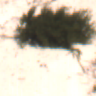
\includegraphics[scale=0.8]{imgs/coast_reduced.png}
    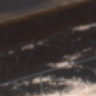
\includegraphics[scale=0.8]{imgs/dsargassum_reduced.png}                
    \caption{Imágenes de $100 \times 100$ pixeles para las clases sargazo, cielo, agua, costa y sargazo muerto respectivamente}
    \label{fig:reduced_images}
\end{figure}

\subsection{Clasificación de imágenes}

Una vez que contamos con el conjunto de entrenamiento y prueba, realizamos una clasificación supervisada de las imágenes de $100\times 100$ pixeles en 5 clases: 
\begin{enumerate}
    \item Sargazo
    \item Sargazo muerto
    \item Agua
    \item Cielo
    \item Costa
\end{enumerate}

Después de realizar esta clasificación, nos quedó la siguiente división:

\begin{table}[H]
    \centering
    \begin{tabular}{|c|c|c|}
    	\hline
		 & Entrenamiento & Prueba \\ \hline
         Sargazo & 134 & 53 \\ \hline
         Sargazo muerto & 128 & 45 \\ \hline
         Agua & 151 & 57 \\ \hline
		 Cielo & 78 & 29 \\ \hline
         Costa & 309 & 116 \\ \hline
         \textbf{Total} & \textbf{800} & \textbf{300} \\ \hline                          
    \end{tabular}
    \caption{Cantidad de imágenes de entrenamiento y prueba divididas en las $5$ clases}
    \label{tab:svd_dimensions}
\end{table}



\subsection{Extracción de características relevantes}

Para la extracción de características, lo que hicimos fue hacer un análisis de texturas con la matriz de co-ocurrencia y las características de Haralick. Las características que seleccionamos para nuestro vector de pruebas fueron las siguientes:

\begin{itemize}
    \item Contraste
    \item Disimilaridad
    \item Homogeneidad
    \item Energía
    \item Correlación
    \item ASM
\end{itemize}


\subsection{Entrenamiento y evaluación de modelos }

Para el entrenamiento y evaluación de modelos, probamos con los siguientes clasificadores:

\begin{itemize}
	\item $k$-vecinos
    \item Máquina de Soporte Vectorial con kernel \textit{rbf}
    \item Clasificador Gausiano de Proceso
    \item Árboles de decisión
    \item \textit{Random Forest}
    \item Perceptrón multi capa
    \item Clasificador \textit{Ada Boost}
    \item Clasificador Bayesiano
    \item Análisis por discriminante cuadrático
\end{itemize}

A continuación se muestran los resultados (precisión) de cada clasificador: 

\begin{figure}[H]
    \centering
    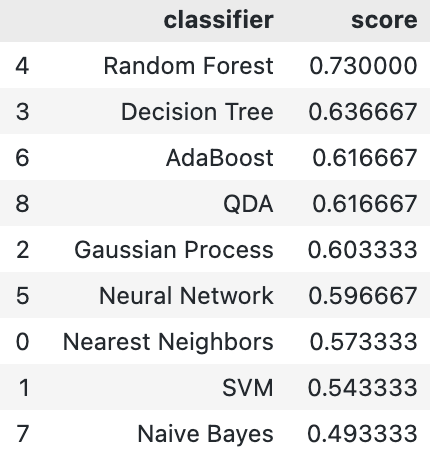
\includegraphics[scale=0.4]{imgs/classifiers_report.png}
    \caption{Reporte de precisión para cada clasificador}
    \label{fig:clfs}
\end{figure}

Podemos observar que el que mejor desempeño tuvo fue el clasificador de árboles aleatorios. Este criterio (precisión) lo tomamos como un valor discriminante para analizar la precisión para la clase \textbf{sargassum} pues el valor mostrado en la figura \ref{fig:clfs} es el promedio general para las $5$ clases. Siguiendo esta lógica, obtuvimos los siguientes resultados:

\begin{itemize}
    \item \textit{Random Forest}:
		\begin{figure}[H]
		    \centering
		    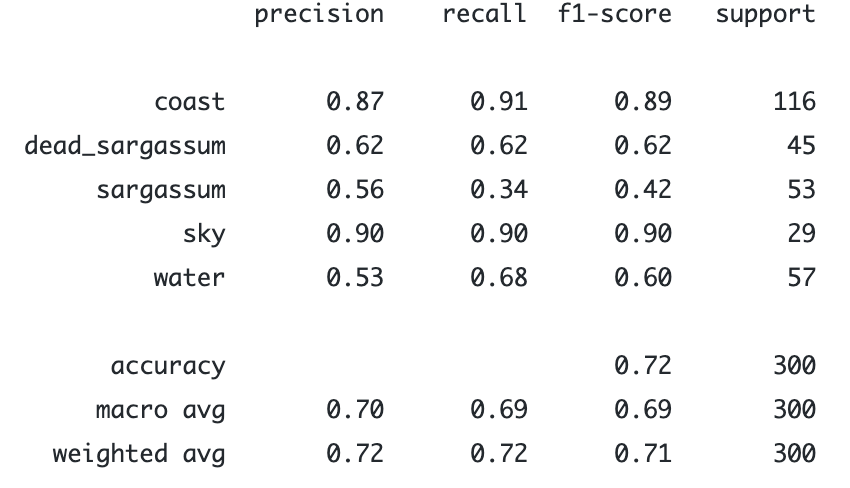
\includegraphics[scale=0.4]{imgs/rf_clasif_report.png}
		    \caption{Reporte de clasificación para \textit{Random Forest}}
		    \label{fig:rf_cr}
		\end{figure}
		
		\begin{figure}[H]
		    \centering
		    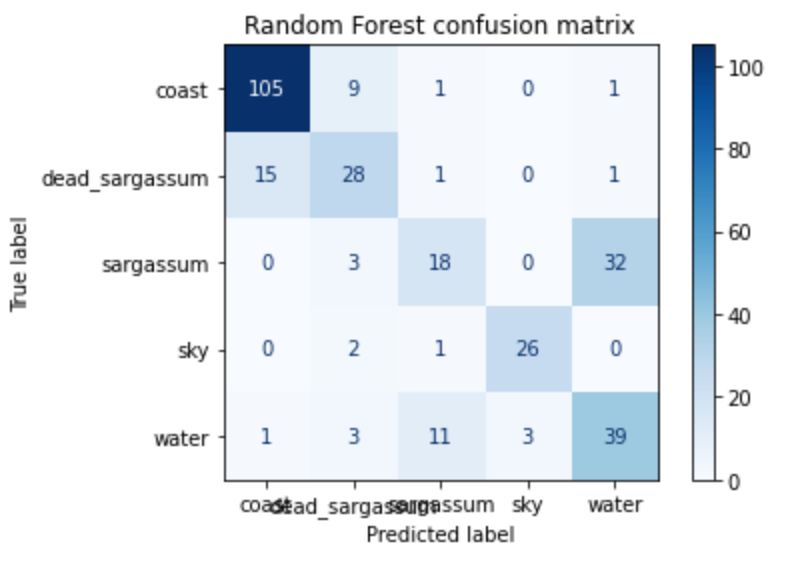
\includegraphics[scale=0.4]{imgs/rf_confusion_mat.png}
		    \caption{Matriz de confusión para \textit{Random Forest}}
		    \label{fig:rf_cm}
		\end{figure}
    \item \textit{Decision Tree}:
		\begin{figure}[H]
		    \centering
		    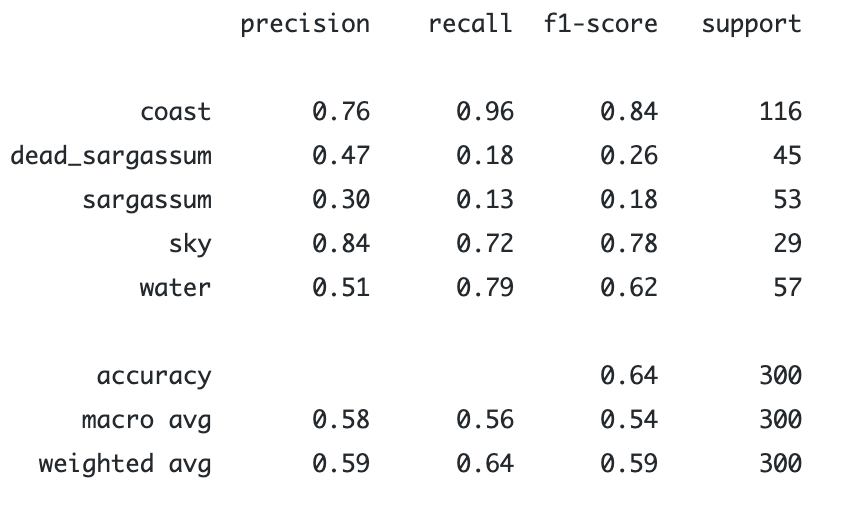
\includegraphics[scale=0.4]{imgs/dt_clasif_report.png}
		    \caption{Reporte de clasificación para \textit{Decision Tree}}
		    \label{fig:dt_cr}
		\end{figure}    

		\begin{figure}[H]
		    \centering
		    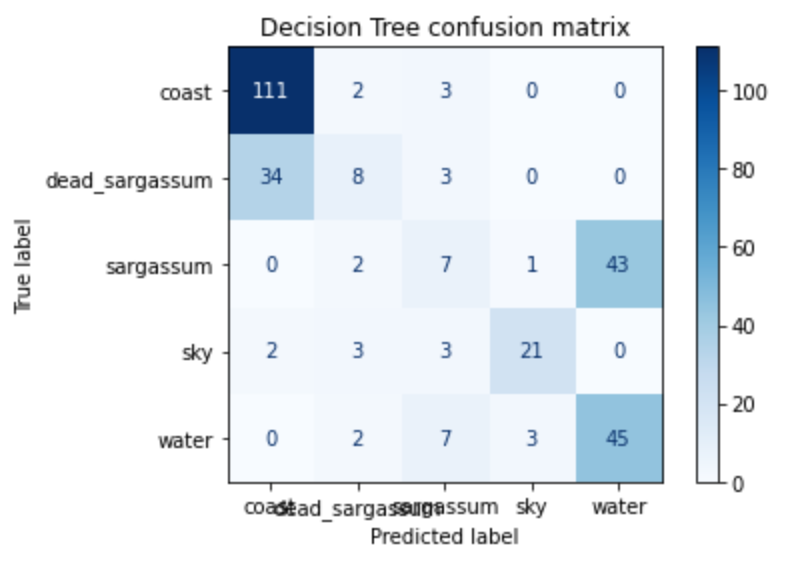
\includegraphics[scale=0.4]{imgs/dt_confusion_mat.png}
		    \caption{Matriz de confusión para \textit{Decision Tree}}
		    \label{fig:dt_cm}
		\end{figure}
		
\end{itemize}


Podemos observar que \textit{Random Forest} a pesar de obtener una precisión de $0.72$, la precisión para el sargazo es de apenas $0.56$. Mientras que para \textit{Decision Tree}, a pesar de obtener una precisión de $0.64$, la precisión de clasificación del sargazo es de apenas $0.3$.


% -------------------------------------------------
% -------------------------------------------------
% -------------------------------------------------
\section{Resultados}


% -------------------------------------------------
% -------------------------------------------------
% -------------------------------------------------
\section{Conclusiones}

Al revisar los resultados 


% -------------------------------------------------
% -------------------------------------------------
% -------------------------------------------------
\section{Secciones de código relevante}
\subsection{Extracción de características}
\begin{lstlisting}[language=python]
def extract_haralick_features(grayscale_image, args):
    distances = args['distances']
    angles = args['angles']
    glcm = greycomatrix(grayscale_image, distances, angles)
    features = [
        np.mean(greycoprops(glcm, 'contrast')),
        np.mean(greycoprops(glcm, 'dissimilarity')),
        np.mean(greycoprops(glcm, 'homogeneity')),
        np.mean(greycoprops(glcm, 'energy')),
        np.mean(greycoprops(glcm, 'correlation')),
        np.mean(greycoprops(glcm, 'ASM')),
    ]
    return features

def label_encode(y):
    le = LabelEncoder()
    le.fit(y)
    return (le.transform(y), le.classes_)

def get_dir_contents(path):
    cts = os.listdir(path)
    return [c for c in cts if c[0] != '.']

def get_X_y_vectors(path, feature_extraction_function, args):
    X = []
    y = []
    for label in get_dir_contents(path):
        for file_name in get_dir_contents(path + label + "/"):
            image = cv2.imread(path + label + "/" + file_name, cv2.IMREAD_GRAYSCALE)
            features = feature_extraction_function(image, args)
            X.append(features)
            y.append(label)
    y, classes_ = label_encode(y)
    return (np.array(X), y, classes_)

#--------------------------------------
#         Feature extraction
#--------------------------------------
TRAIN_IMAGES_PATH = 'dataset/train/'
TEST_IMAGES_PATH = 'dataset/test/'

haralick_args = {
    'distances': [1], 
    'angles': [0, np.pi/4, np.pi/2, 3*np.pi/4]
}

X_train, y_train, train_classes_ = get_X_y_vectors(
    TRAIN_IMAGES_PATH, extract_haralick_features, haralick_args
)
X_test, y_test, test_classes_ = get_X_y_vectors(
    TEST_IMAGES_PATH, extract_haralick_features, haralick_args
)


print(f"X_train: {X_train.shape}\ty_train: {y_train.shape}")
print(f"X_test: {X_test.shape}\ty_test: {y_test.shape}")
print(f"Train classes: {train_classes_}\nTest classes: {test_classes_}")\end{lstlisting}


\subsection{Entrenamiento de clasificadores}

\begin{lstlisting}[language=python]
#--------------------------------------
#     Model training and evaluation
#--------------------------------------
classifiers = [
    KNeighborsClassifier(n_neighbors=5, weights='distance'),
    SVC(),
    GaussianProcessClassifier(),
    DecisionTreeClassifier(max_depth=5),
    RandomForestClassifier(),
    MLPClassifier(alpha=1, max_iter=1000),
    AdaBoostClassifier(random_state=0),
    GaussianNB(),
    QuadraticDiscriminantAnalysis()
]
names = ["Nearest Neighbors", "SVM", "Gaussian Process",
         "Decision Tree", "Random Forest", "Neural Network", "AdaBoost",
         "Naive Bayes", "QDA"]

scores = []

for name, classifier in zip(names, classifiers):
    classifier.fit(X_train, y_train)
    score = classifier.score(X_test, y_test)
    y_pred = classifier.predict(X_test)
    scores.append(score)

df = pd.DataFrame({'classifier': names,'score': scores})
df = df.sort_values(by='score', ascending=False)\end{lstlisting}

\subsection{Evaluación de modelos}
\begin{lstlisting}[language=python]
#--------------------------------------
#         Confusion matrix
#--------------------------------------
def evaluate(model, X_test, y_true, y_pred, target_names, model_name):
    print(f"{model_name}")
    print(classification_report(y_true, y_pred, target_names=target_names))
    plot_confusion_matrix(
        model, X_test, y_true, display_labels=target_names, cmap=plt.cm.Blues
    )
    plt.title(f"{model_name} confusion matrix")
    plt.show()
    
best_classifiers_df = df.iloc[:2]
for idx in np.array(best_classifiers_df.index):
    name = names[idx]
    clf = classifiers[idx]
    clf.fit(X_train, y_train)
    y_pred = clf.predict(X_test)
    evaluate(clf, X_test, y_test, y_pred, test_classes_, name)\end{lstlisting}




% -------------------------------------------------
% -------------------------------------------------
% -------------------------------------------------
\selectlanguage{spanish}
\begin{thebibliography}{}
\bibitem{}

\end{thebibliography}

\end{document}
